\chapter{Narzędzia i zewnętrzne biblioteki}

\section{Docker}

\subsection[Czym jest docker?]{Czym jest docker?}
\par{Docker jest narzędziem przeznaczonym do tworzenie przenośnych, wirtualnych kontenerów pozwalających na prostą i szybką replikację środowiska.}

\par{Oprogramowanie Docker wprowadza standaryzację w środowisko uruchomieniowe. Generowane kontenery są spójne i takie same w różnych środowiskach. W chwili obecnej Docker wymaga jądra Linux do uruchomienia, jednak działa nie tylko w wersji natywnej, ale również poprzez wirtualizację specjalnych minimalistycznych dystrybucji Linux na systemach Mac OS X oraz Windows (na przykład w darmowym narzędziu do wirtualizacji – VirtualBox).}

\subsection[Spójność]{Spójność}

\par{Docker wprowadzenie spójność w środowisko deweloperskie. Często, kiedy nad projektem pracuje więcej niż jeden programista (co w dzisiejszych czasach jest normą) pojawia się problem z różnymi wersjami użytego oprogramowania. Zdarza się, że jedna wersja biblioteki zachowuje się inaczej od drugiej (na przykład z powodu błędu). Kontener z założenia posiada jedną, konkretną wersję każdej biblioteki koniecznej do uruchomienie aplikacji. Zwiększa to przewidywalność oprogramowania. Oczekujemy bowiem, że w tym samym środowisku, aplikacja będzie zachowywać się tak samo. }

\subsection[Cykl Dockera]{Cykl Dockera}


\begin{enumerate}
\item Stworzenie kontenera wraz z wszelkimi narzędziami i bibliotekami koniecznymi do uruchomienia aplikacji. 
\item Rozprowadzenie kontenera, wraz ze wszystkimi narzędziami i bibliotekami. 
\item Uruchomienie identycznego kontenera na dowolnej liczbie węzłów. 
\end{enumerate}

\par{Prowadzi to do znacznych ułatwień w tworzeniu oprogramowania. Ten sam kontener może zostać rozprowadzony pomiędzy deweloperami, testerami, serwerami ciągłej integracji i w końcu środowiskiem produkcyjnym. }

\subsection[Centralne repozytorium]{Centralne repozytorium}

\par{Każdy zarejestrowany użytkownik ma możliwość wgrywania własnych kontenerów do centralnego, ogólnie dostępnego repozytorium. Można tam znaleźć wiele różnych gotowych obrazów do pobrania. Są one przygotowane zarówno przez społeczność jak i przez twórców Dockera. }

\par{Centralne repozytorium pozwala użytkownikom na pobranie interesujących obrazów, szczególnie warte uwagi są repozytoria przygotowane pod konkretne rozwiązania (na przykład specjalnie pod serwer baz danych MySQL lub mongoDB). }

\par{Docker umożliwia również stworzenie prywatnych repozytoriów. Dzięki temu nie musimy upubliczniać prywatnych obrazów, ale jednocześnie możemy je rozprowadzać. Inną dostępną metodą jest zapis obrazu do pliku i przekazanie go w tradycyjny sposób. }

\subsection[Przeprowadzone testy]{Przeprowadzone testy}

W ramach zapoznania się z platformą Docker wykonaliśmy następujące czynności: 
\begin{itemize}

\item Zweryfikowaliśmy możliwość uruchomienia oprogramowania na systemach operacyjnych Ubuntu oraz Mac OS X. 


\item Na systemie Max OS X skorzystaliśmy z programu Boot2Docker, tworzącego maszynę wirtualną z minimalistyczną dystrybucją Linux konieczną do uruchomienia aplikacji Docker.

\begin{figure}[h]
\begin{center}
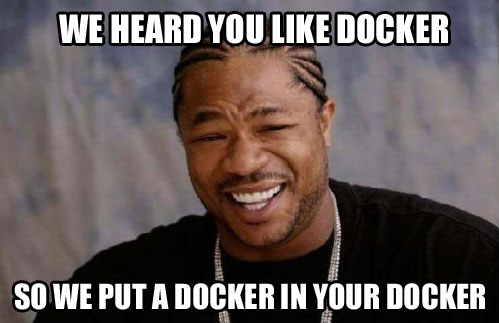
\includegraphics[width=0.8\linewidth]{img/docker_tut1.jpg} 
\caption{Skorzystanie z programu Boot2Docker}
\label{img:docker_tut1}
\end{center}
\end{figure}

\item Pobraliśmy obraz Systemu operacyjnego Ubuntu, na którym zainstalowaliśmy programy nginx oraz vim. 

\item Przy pomocy programu vim, zmodyfikowaliśmy treść domyślnego pliku index.html, który dostępny jest na porcie 80 po uruchomieniu programu nginx. 

\item Zweryfikowaliśmy zmianę w przeglądarce internetowej. 

\item Zapisaliśmy zmiany w kontenerze oraz wgraliśmy zmieniony obraz do centralnego repozytorium. 

\item Pobraliśmy obraz na innym komputerze i po uruchomieniu zweryfikowaliśmy zmiany wprowadzone do podstawowej dystrybucji Ubuntu. 

\item W pobranym obrazie zainstalowane były programy nginx oraz vim. Domyślny plik programu nginx był również zmodyfikowany. 

\end{itemize}

\section[IDE IntelliJ]{IDE IntelliJ}

\subsection*[Powody wyboru biblioteki]{Powody wyboru biblioteki}

\section{Google Protocol Buffers} \label{protobuf}

\par{Jest to elastyczna i wydajna metoda serializacji strukturyzowanych danych do wykorzystania między innymi w protokołach komunikacyjnych oraz przechowywaniu danych. Określana jest struktura informacji która będzie serializowana poprzez zdefiniowanie typu wiadomości w pliku ,,.proto''. Każda taka wiadomość jest logicznym rekordem informacji zawierającym pary nazwa-wartość. Format takiej wiadomości jest prosty, każdy typ składa się z jednego lub więcej unikatowych, ponumerowanych pól z których każdy ma nazwę i typ wartości. Typem wartości pola mogą być liczby, zmienne logiczne, łańcuchy znaków oraz inne wiadomości PBM. Pozwala to na hierarchiczne ułożenie struktury. Każde pole może być oznaczone na trzy sposoby: opcjonalne, wymagane, powtarzające się z zachowaniem kolejności.}

\par{Kiedy wiadomości są określone należy włączyć kompilator protocol buffer dla języka aplikacji. Generuje on klasy dostępu do danych na podstawie pliku ,,.proto''. Tworzone są podstawowe funkcje dostępu do każdego pola oraz metody do serializowania/parsowania całej struktury. Dla Javy generowane są pliki ,,.java'' z klasami dla każdego typu wiadomości oraz specjalna klasa ,,Builder'' do tworzenia instancji klas wiadomości.}

\par{Można dodać nowe pola do wiadomości nie zaburzając kompatybilności wstecznej. Stare pliki binarne ignorują nowe pola podczas parsowania. W przypadku protokołów komunikacyjnych które wykorzystują protocol buffers jako format danych, można rozszerzyć protokół bez obaw o wpływ na istniejący kod.}

\subsection*[Powody wyboru biblioteki]{Powody wyboru biblioteki}
